En esta sección se presentan los resultados de ambos enfoques algorítmicos mediante gráficos de dispersión, considerando los costos y archivos de entrada disponibles en el repositorio de GitHub referenciado en la sección de Implementación. Cabe destacar que estos archivos no han sido ni serán modificados, lo que permite verificar la reproducibilidad de los resultados.

Para replicar los experimentos, basta con ejecutar los comandos \texttt{make} mencionados anteriormente, ingresando manualmente los datos de entrada que se encuentran en los archivos \texttt{.txt}. Aunque sería posible automatizar todos los casos mediante \texttt{make}, esto haría el proceso innecesariamente complejo y menos flexible para el usuario, limitando la posibilidad de probar casos específicos de forma manual. Para detalles sobre la compilación y ejecución de los programas \texttt{.cpp}, puede utilizar el comando \textbf{\texttt{make help}} en la terminal. Es importante asegurarse de que el sistema tenga un compilador compatible con archivos \texttt{.cpp} y soporte para \texttt{make}, de lo contrario, los comandos no funcionarán correctamente.

En la \cref{fig:grafico_dispersion_1}, se presentan los resultados obtenidos al ejecutar los cinco casos del dataset \textit{transpose}. La gráfica muestra un claro crecimiento exponencial en el tiempo de ejecución del algoritmo basado en \textit{Fuerza Bruta} (puntos en color azul), mientras que el enfoque de \textit{Programación Dinámica} (puntos en color naranja) mantiene un crecimiento lineal. Se observa un caso anómalo cuando la longitud de \( S1 \) es 5, lo cual podría ser explicado por variaciones en la gestión de memoria o costos específicos.

\begin{figure}[H]
    \centering
    
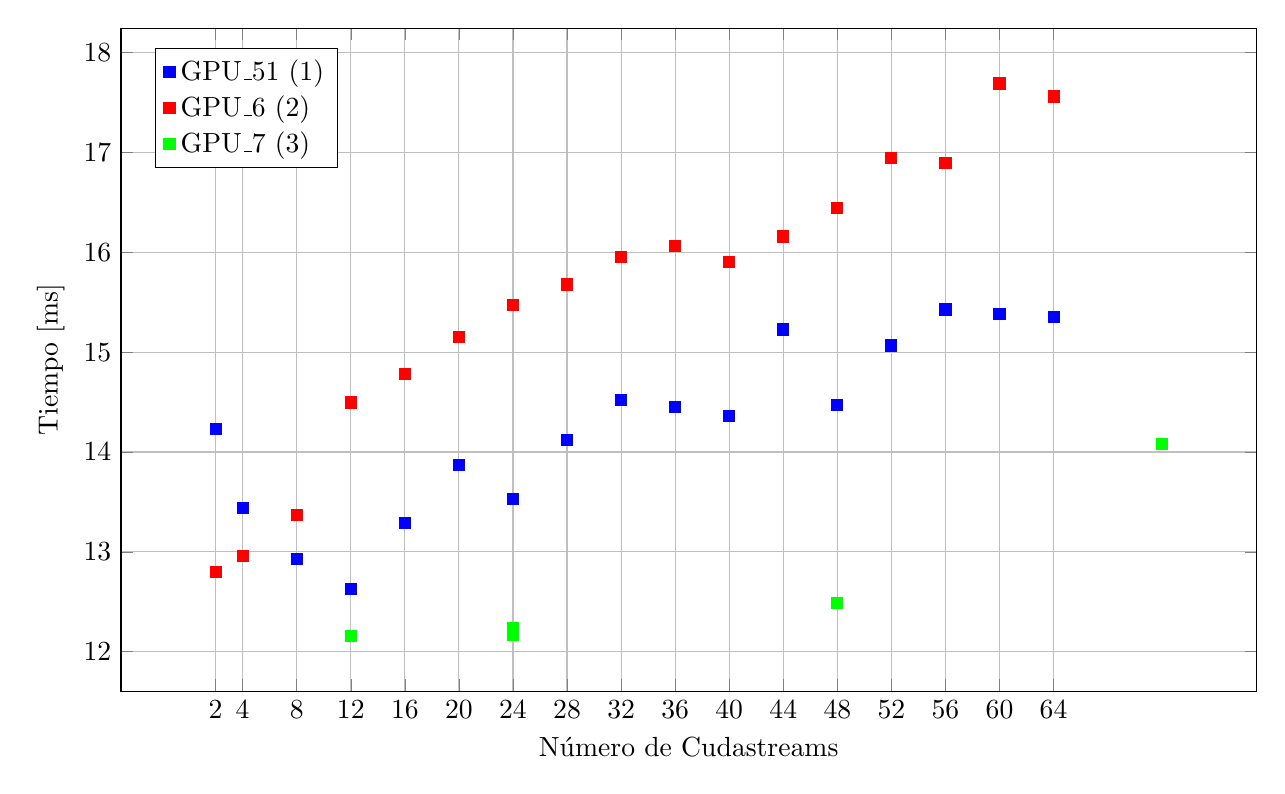
\begin{tikzpicture}
    %\begin{loglogaxis}[
    %\begin{semilogxaxis}[ % Cambiar a semilogxaxis    
    \begin{axis}[
        xlabel={Número de Cudastreams },
        ylabel={Tiempo [ms]},
        grid=major,
        legend pos=north west,
        legend cell align={left},
        width=16cm,
        height=10cm, 
        xtick=data,
    ]
    \addplot[blue, only marks, mark=square*] coordinates {
        (2   , 14.229344)
        (4   , 13.435616 )
        (8   , 12.929280 )
        (12  , 12.628000 )
        (16  , 13.286176 )
        (20  , 13.873152 )
        (24  , 13.531168 )
        (28  , 14.116384 )
        (32  , 14.518528 )
        (36  , 14.448992 )
        (40  , 14.356640 )
        (44  , 15.226560 )
        (48  , 14.473888 )
        (52  , 15.066720 )
        (56  , 15.426560 )
        (60  , 15.380416 )
        (64  , 15.348064 )
    };
    \addlegendentry{GPU\_51 (1)}
    \addplot[red, only marks, mark=square*] coordinates {
        (2  , 12.799264 ) 
        (4  , 12.956192 )
        (8  , 13.371104 )
        (12 , 14.495616 )
        (16 , 14.783360 ) 
        (20 , 15.152672 ) 
        (24 , 15.475488 ) 
        (28 , 15.676416 ) 
        (32 , 15.948800 ) 
        (36 , 16.064129 ) 
        (40 , 15.904544 ) 
        (44 , 16.157921 ) 
        (48 , 16.444992 ) 
        (52 , 16.943169 ) 
        (56 , 16.894304 ) 
        (60 , 17.689600 ) 
        (64 , 17.559551 ) 
    };
    \addlegendentry{GPU\_6 (2)}
    \addplot[green, only marks, mark=square*] coordinates {
        (6, 17.607168) 
        (12, 12.159264) 
        (24, 12.239648) 
        (24, 12.169376) 
        (48, 12.490624) 
        (72, 14.081920) 
    };
    \addlegendentry{GPU\_7 (3)}
   
\end{axis}
%\end{semilogxaxis} % Cambiar a semilogxaxis
\end{tikzpicture}

    \caption{Gráfica de dispersión para \textit{transpose dataset}, contrastando el uso del enfoque de fuerza bruta y el de programación dinámica.}
    \label{fig:grafico_dispersion_1}
\end{figure}

En las siguientes figuras (\cref{fig:grafico_dispersion_2} y \cref{fig:grafico_dispersion_3}), se muestran los resultados obtenidos para los datasets \textit{semiordered} y \textit{disordered}. En ambos casos, se observa un comportamiento similar al descrito anteriormente: los tiempos de ejecución dependen principalmente de la longitud de \( S1 \). Esto es consistente independientemente de si las cadenas están parcialmente ordenadas o completamente desordenadas. 

El rendimiento del algoritmo mejora significativamente en casos donde:
\begin{enumerate}
    \item \( S1 \) y \( S2 \) comparten una gran cantidad de caracteres en las mismas posiciones.
    \item Uno de los strings está vacío o es considerablemente más corto que el otro.
\end{enumerate}

Estos escenarios representan casos interesantes para probar ambos enfoques, y se invita al lector a explorar estas posibilidades para comprender mejor las fortalezas y limitaciones de cada algoritmo.

\begin{figure}[H]
    \centering
    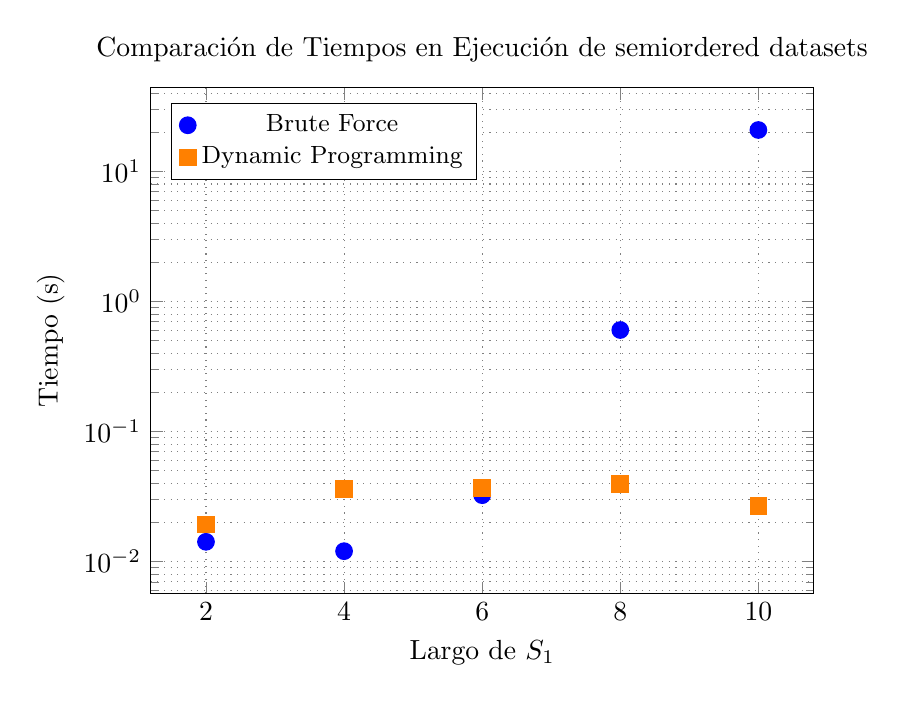
\begin{tikzpicture}
    \begin{axis}[
        ylabel={Tiempo (s)},
        xlabel={Largo de $S_1$},
        title={Comparación de Tiempos en Ejecución de semiordered datasets},
        legend pos=north west,
        ymode=log, % Escala logarítmica para resaltar diferencias de tiempo
        grid=both,
        grid style={dotted, gray},
        legend style={font=\small},
        width=10cm,
        height=8cm
    ]

    % Datos de brute force (color azul)
    \addplot[
        only marks,
        mark=*,
        color=blue,
        mark options={scale=1.5}
    ] coordinates {
        (2, 0.014218)
        (4, 0.012048)
        (6, 0.032464)
        (8, 0.603942)
        (10, 20.8217)
    };
    \addlegendentry{Brute Force}

    % Datos de dynamic programming (color naranja)
    \addplot[
        only marks,
        mark=square*,
        color=orange,
        mark options={scale=1.5}
    ] coordinates {
        (2, 0.019347)
        (4, 0.036098)
        (6, 0.036963)
        (8, 0.039428)
        (10, 0.026698)
    };
    \addlegendentry{Dynamic Programming}

    \end{axis}
\end{tikzpicture}
    \caption{Gráfica de dispersión para \textit{semiordered dataset}, contrastando el uso del enfoque de fuerza bruta y el de programación dinámica.}
    \label{fig:grafico_dispersion_2}
\end{figure}

\begin{figure}[H]
    \centering
    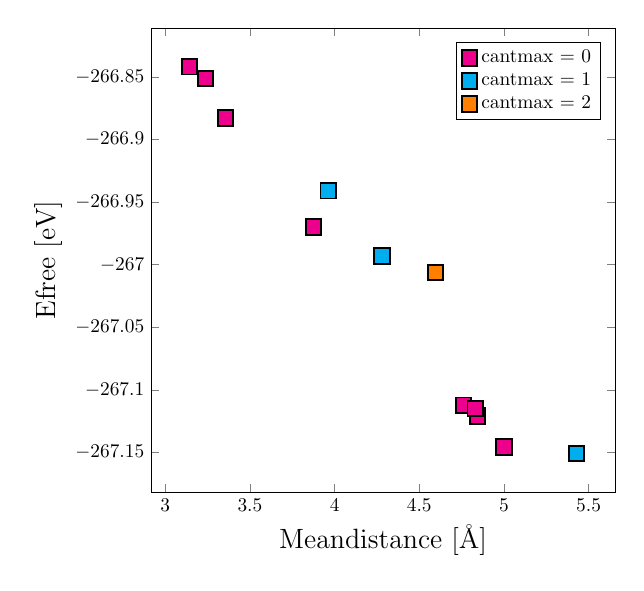
\begin{tikzpicture}[scale=0.7]
    %\begin{loglogaxis}[
    %\begin{semilogxaxis}[ % Cambiar a semilogxaxis    
    \begin{axis}[
        xlabel={\Large Meandistance [\AA] },
        ylabel={\Large Efree [eV]},
        %grid=major,
        legend pos=north east,
        legend cell align={left},
        %log basis x=10,
        %log basis y=10,
        %xmin=2, xmax=2^21,
        %ymin=0.1, ymax=100,
        width=10cm, % Ajusta el ancho de la gráfica
        height=10cm, % Ajusta la altura de la gráfica
        %xtick=data,
    ]
    \addplot[magenta , only marks, mark=square*, mark options={draw=black,line width = 1pt}, mark size=4pt] coordinates {
        (4.845001   ,	-267.121023)	% 0
        (5.000617   ,	-267.145714)	% 0
        (4.760055   ,	-267.112360)	% 0
        (3.236691   ,	-266.851158)	% 0
        (3.356972   ,	-266.882713)	% 0
        %(5.427886   ,	-267.150822)	% 1
        (4.830514   ,	-267.115114)	% 0
        (3.144397   ,	-266.841800)	% 0
        %(4.280839   ,	-266.992946)	% 1
        (3.874418   ,	-266.969850)	% 0
        %(4.595953   ,	-267.006159)	% 2
        %(3.962469   ,	-266.940902)	% 1       
        };
    \addlegendentry{cantmax = 0} 
    \addplot[cyan , only marks, mark=square*, mark options={draw=black,line width = 1pt}, mark size=4pt] coordinates {
        (5.427886   ,	-267.150822)	% 1
        (4.280839   ,	-266.992946)	% 1
        (3.962469   ,	-266.940902)	% 1
        };
        \addlegendentry{cantmax = 1} 
    \addplot[orange , only marks, mark=square*, mark options={draw=black,line width = 1pt}, mark size=4pt] coordinates {
        (4.595953   ,	-267.006159)	% 2
        };
        \addlegendentry{cantmax = 2}
\end{axis}
%\end{semilogxaxis} % Cambiar a semilogxaxis
\end{tikzpicture}
    \caption{Gráfica de dispersión para \textit{disordered dataset}, contrastando el uso del enfoque de fuerza bruta y el de programación dinámica.}
    \label{fig:grafico_dispersion_3}
\end{figure}

Finalmente, para replicar las gráficas presentadas, puede modificar las tuplas en la sección \textit{tikz} del tarball proporcionado, o bien, utilizar herramientas como Excel para generar automáticamente gráficos de dispersión ingresando los mismos datos. Esta última opción puede ser más conveniente si no está trabajando estrictamente con \LaTeX.
